\documentclass{article}
\usepackage{../../mypackages}
\usepackage{../../macros}

% Variable de correction


% Variable de correction
% \newif\ifWITHCORRECTION
% \WITHCORRECTIONtrue % Mettre \WITHCORRECTIONfalse pour la version élève

% Commandes pour masquer du texte en fonction de la version
%\newcommand{\corrige}[2]{\ifWITHCORRECTION #1 \else \underline{\hspace{#2}} \fi}


\def\WITH_CORRECTION{NO}

\title{Chapitre 2 - Les Matériaux Organiques}
\author{N. Bancel}
\date{Septembre 2024}

\renewcommand{\arraystretch}{2} % Increases row height by 2x

\begin{document}

\maketitle

% Rappels de 2nde

\section{Attendus de fin de chapitre}


\begin{tcolorbox}[colback=red!10!white, colframe=red!75!black, title="Ce qu'il faut à tout prix retenir / savoir faire"]
  \begin{itemize}[noitemsep]
    \item Bien comprendre le principe d'électrons de valence, de couche de valence. 
    \item Connaître et comprendre la règle du duet et de l'octet
    \item Etre en mesure d'écrire une configuration électronique, et d'en déduire le nombre de doublets non-liants et de doublants liants afin de satisfaire la règle du duet ou de l'octet 
    \item Schéma de Lewis d'un atome 
    \item Formule brute, développée, semi-developpée d'une molécule.
    \item Connaître la définition d'un alcane, d'un alcène, d'un composé aromatique 
    \item Connaître les groupes caractéristiques de l'alcool, l'acide carbonxylique, esther
    \item Définition d'un polymère
    \item Identifier une polycondensation, et une polyaddition
    \item \textbf{En gros, à partir du dessin de n'importe quelle molécule organique, être capable d'écrire sa formule brute, développée, semi-développée, déterminer son groupe caractéristique, et si c'est un alcène, un alcane, un composé aromatique, un polymère et}
  \end{itemize}

\end{tcolorbox}


\section{Rappels de 2nde}

\subsection{Couches électroniques et électrons de valence}

\begin{tcolorbox}[colback=green!10!white, colframe=green!75!black, title=Définitions : ]
  Les électrons se répartissent autour du noyau atomique selon des couches électroniques et des sous-couches. \par 
  \vspace{1em}
  Les \textbf{couches électroniques} sont notées \(n = 1, 2, 3\) etc \par 
  Chaque couche électronique est divisée en \textbf{sous-couches} qui sont notées par les lettres \(s\), \(p\), etc.
  \begin{itemize}[noitemsep]
    \item La sous-couche \(s\) peut contenir jusqu'à 2 électrons.
    \item La sous-couche \(p\) peut contenir jusqu'à 6 électrons.
  \end{itemize}

  Dans la configuration électronique à l'état fondamental d'un atome de numéro atomique inférieur ou égal à 18, les électrons \textit{ns} et \textit{np} associés à la plus grande valeur de \textit{n} sont appelés \textbf{électrons de valence}
  
  Seuls les électrons de la couche externe (électrons de valence) participent aux liaisons entres atomes dans les molécules, ou à la formation d'ions. 
  
\end{tcolorbox}

\begin{tcolorbox}[colback=blue!10!white, colframe=blue!75!black, title=Application : Structure électronique]
  Exemple de l'atome d'oxygène (O) : Numéro atomique : \(Z = 8\) \\
  Sa configuration électronique est : \(1s^2 2s^2 2p^4\). \\
  Cela signifie :
  \begin{itemize}[noitemsep]
    \item 2 électrons dans la première couche (1s$^2$)
    \item 2 électrons dans la sous-couche s de la deuxième couche (2s$^2$)
    \item 4 électrons dans la sous-couche p de la deuxième couche (2p$^4$)
  \end{itemize}
  Il possède donc 6 électrons de valence (2s$^2$ 2p$^4$).
\end{tcolorbox}

\vspace{1em}


\subsection{Stabilité}

\begin{tcolorbox}[colback=red!10!white, colframe=red!75!black, title=Important]
\textbf{Règle de stabilité} : au cours des transformations chimiques, les atomes acquièrent la même configuration électronique que celle d'un atome de gaz noble, c'est-à-dire une configuration électronique de valence en duet ou en octet. \par
\vspace{1em}
Ils cherchent à obtenir une couche de valence \textbf{remplie}. Composée donc de soit 2 électrons, soit 8 électrons
\end{tcolorbox}

\begin{tabularx}{\linewidth}{|| p{2.5cm} | p{1.5cm} | X | p{3cm} | X ||}
  \toprule
  {Atome} & {Numéro atomique} & {Configuration électronique} & {\# électrons nécessaires pour remplir la couche de valence ?} & {Gaz noble ?} \\
  \midrule
  {Hélium (\ce{He})} & {2} & {$1s^2$} & {0} & {Oui} \\ 
  {Carbone (\ce{C})} & {6} & {$1s^2 2s^2 2p^2$} & {4} & {Non} \\ 
  {Néon (\ce{Ne})} & {10} & {$1s^2 2s^2 2p^6$} & {0} & {Oui} \\
  {Oxygène (\ce{O})} & {8} & {$1s^2 2s^2 2p^4$} & {2} & {Non} \\ 
  {Argon (\ce{Ar})} & {18} & {$1s^2 2s^2 2p^6 3s^2 3p^6$} & {0} & {Oui} \\
  {Azote (\ce{N})} & {7} & {$1s^2 2s^2 2p^3$} & {3} & {Non} \\ 
  {Hydrogène (\ce{H})} & {1} & {$1s^1$} & {1} & {Non} \\
  {Chlore (\ce{Cl})} & {17} & {$1s^2 2s^2 2p^6 3s^2 3p^5$} & {1} & {Non} \\ 
  \bottomrule
\end{tabularx}

\subsection{Stabilité chimique et liaisons chimiques}

\subsubsection{Couche de valence}

\begin{figure}[H]
  \centering
  \includegraphics[width=\linewidth]{stabilité_chimique.jpg}
  \caption{\label{} Stabilité chimique}
\end{figure}



\begin{tcolorbox}[colback=green!10!white, colframe=green!75!black, title=Définitions : ]
  Dans une molécule, les atomes mettent des électrons de valence en commun avec d'autres atomes afin d'obtenir la configuration électronique de valence en duet ou en octet. \par
  \vspace{1em}
  La mise en commun de deux électrons de valence par deux atomes permet la réalisation d'une liaison chimique.
  \vspace{1em}
  Plus familièrement : \textit{"Si je prends un électron, j'en donne un"}
\end{tcolorbox}

\subsubsection{Les doublets liants / non liants}

Dans une molécule, les atomes possèdent sur leur couche électronique de valence deux types de doublets électroniques (paquet de deux électrons).
\begin{itemize}[noitemsep]
  \item Les doublets liants constituent les liaisons chimiques réalisées avec d'autres atomes.
  \item Les doublets non liants appartiennent uniquement à l'atome
\end{itemize}

\subsubsection{Les doublets liants / non liants}

\begin{figure}[H]
  \centering
  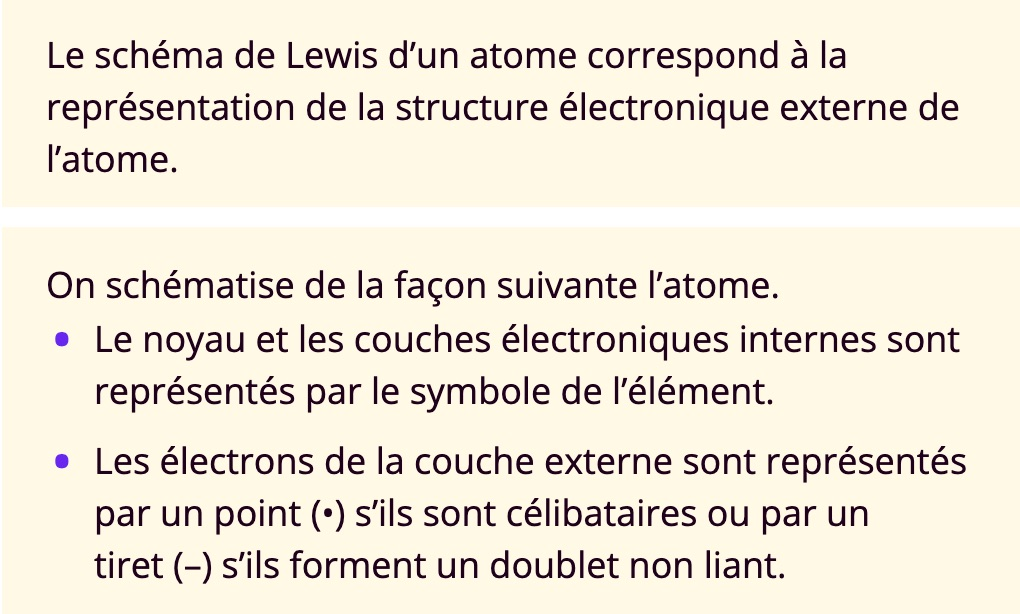
\includegraphics[width=0.6\linewidth]{lewis.jpg}
  \caption{\label{} Schéma de Lewis}
\end{figure}


\begin{tabular}{|| p{3cm} | p{6cm} | p{4cm} ||}
  \toprule
  {Atome} & {Nombres d'électrons "célibataires" / ayant besoin de se lier avec l'électron d'un autre atome} & {Schéma de Lewis} \\
  \midrule
  {Hydrogène (\ce{H})} & {} & {} \\
  {Carbone (\ce{C})} & {} & {} \\ 
  {Azote (\ce{N})} & {} & {} \\ 
  {Oxygène (\ce{O})} & {} & {} \\ 
  {Chlore (\ce{Cl})} & {} & {} \\ 
  \bottomrule
\end{tabular}

\vspace{1em}
\textcolor{blue}{\textbf{Réponses}}
\vspace{1em}

\begin{figure}[H]
  \centering
  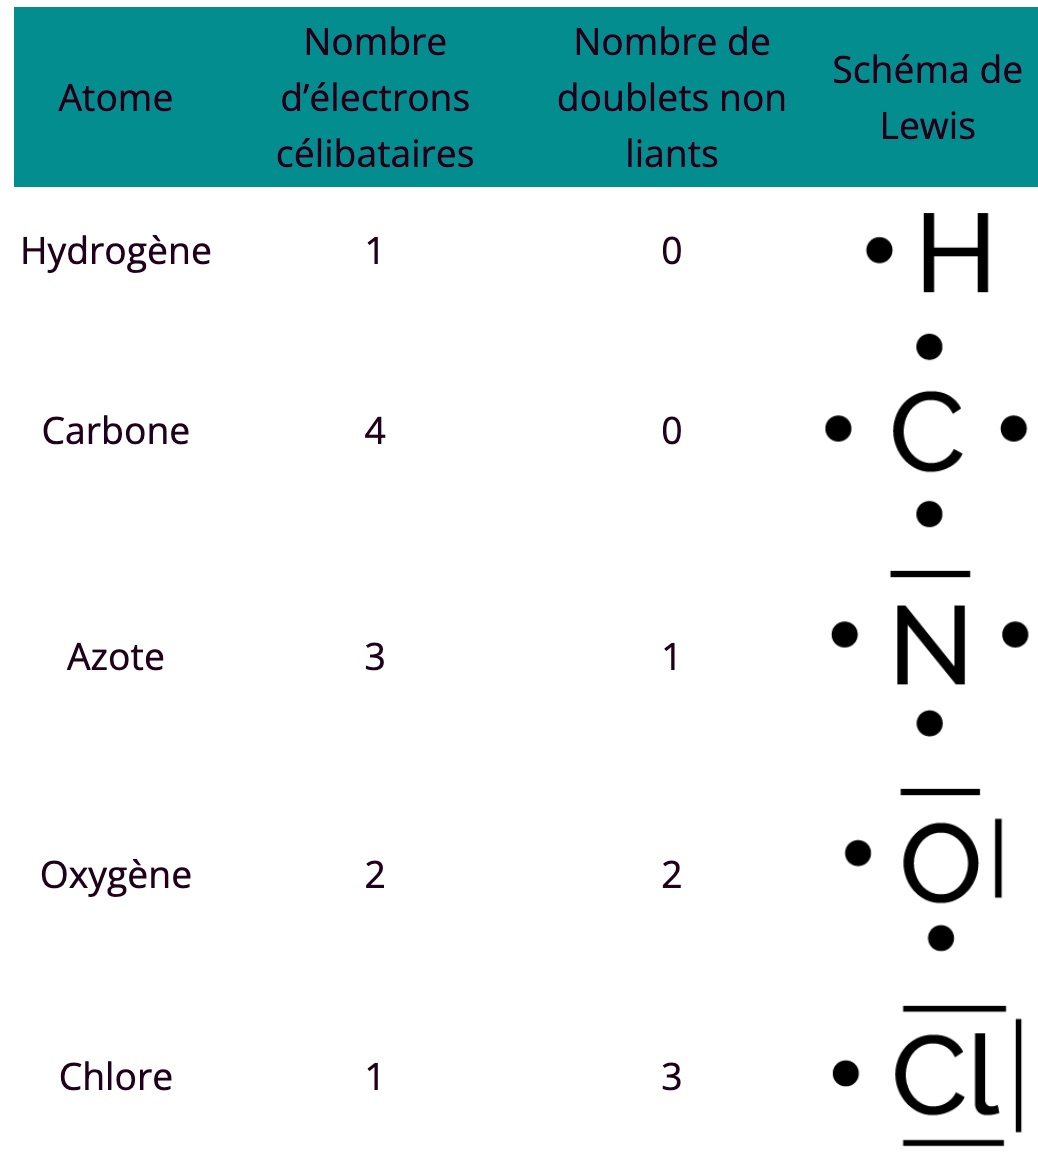
\includegraphics[width=0.8\linewidth]{lewis_reponses.jpg}
  \caption{\label{} Schémas de Lewis}
\end{figure}


\subsubsection{Exemples d'application + Représenttion des molécules}

Le schéma de Lewis d'une molécule correspond à la représentation des atomes qui constituent la molécule et de leurs doublets liants et non liants. \par
\vspace{1em}
On représente un doublet liant par un tiret entre les deux atomes liés, et un doublet non liant par un tiret à côté de l'atome. \par
\vspace{1em}
En s'aidant des tableaux remplis au-dessus, et du cours, dessiner le schéma de Lewis des molécules suivantes 

\begin{itemize}[noitemsep]
  \item Eau : \ce{H2O}
  \item Méthane : \ce{CH4}
  \item Ammoniac : \ce{NH3}
  \item Dioxygène : \ce{O2}
  \item Dioxyde de carbone : \ce{CO2}
\end{itemize}

Réponses : 

\begin{tabular}{|| >{\centering\arraybackslash}p{3cm} | >{\centering\arraybackslash}p{6cm} | >{\centering\arraybackslash}p{4cm} ||}
  \toprule
  {Nom de molécule} & {Formule brute} & {Schema de Lewis} \\
  \midrule
  {Eau} & {\ce{H2O}} & {\chemfig{H-[:30]O-[:-30]H}} \\
  {Méthane} & {\ce{CH4}} & {{\chemfig{H-C(-[2]H)(-[6]H)-H}}} \\[4em]
  {Ammoniac} & {\ce{NH3}} & {\chemfig{H-N(-[2]H)-H}} \\
  {Dioxygène} & {\ce{O2}} & {\chemfig{O=O}} \\
  {Dioxyde de carbone} & {\ce{CO2}} & {\chemfig{O=C=O}} \\
  \bottomrule
\end{tabular}



\section{Les chaînes carbonées}

\subsection{L'atome de carbone}

\begin{figure}[H]
  \centering
  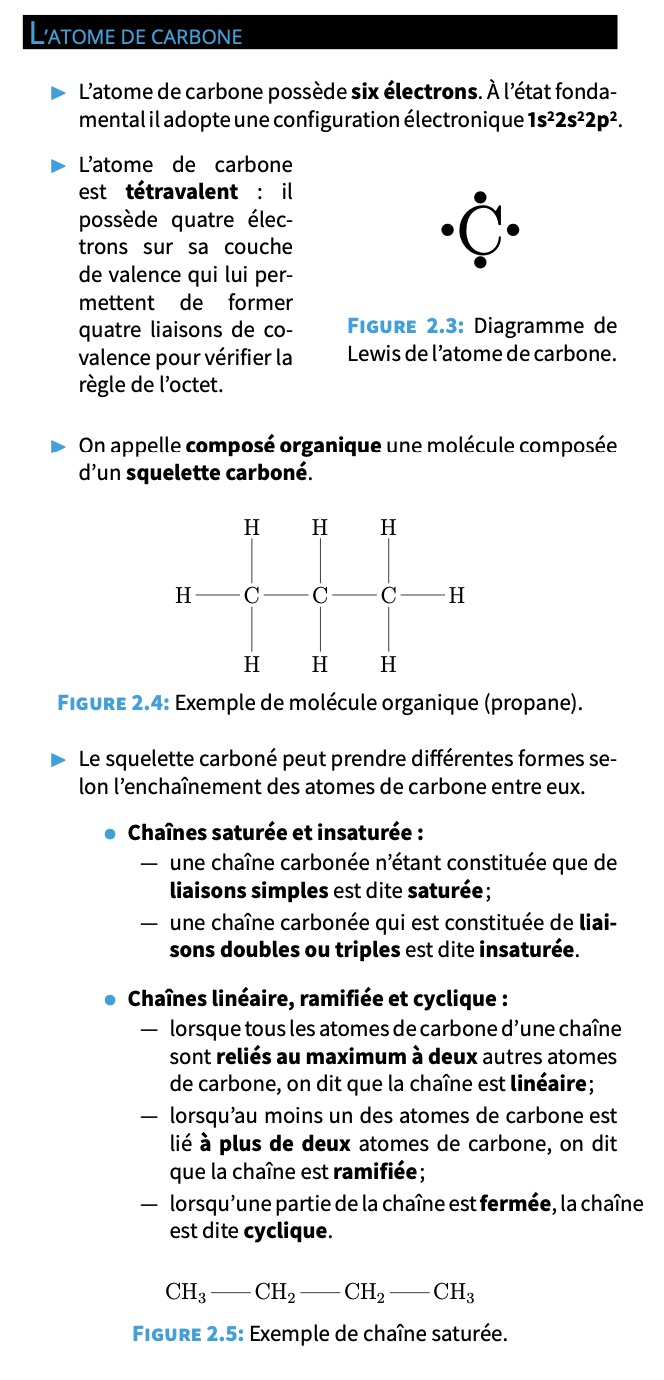
\includegraphics[width=0.6\linewidth]{livre_page1.jpg}
  \caption{\label{} Chaînes carbonées}
\end{figure}

\subsection{Modélisation de molécules}

\begin{figure}[H]
  \centering
  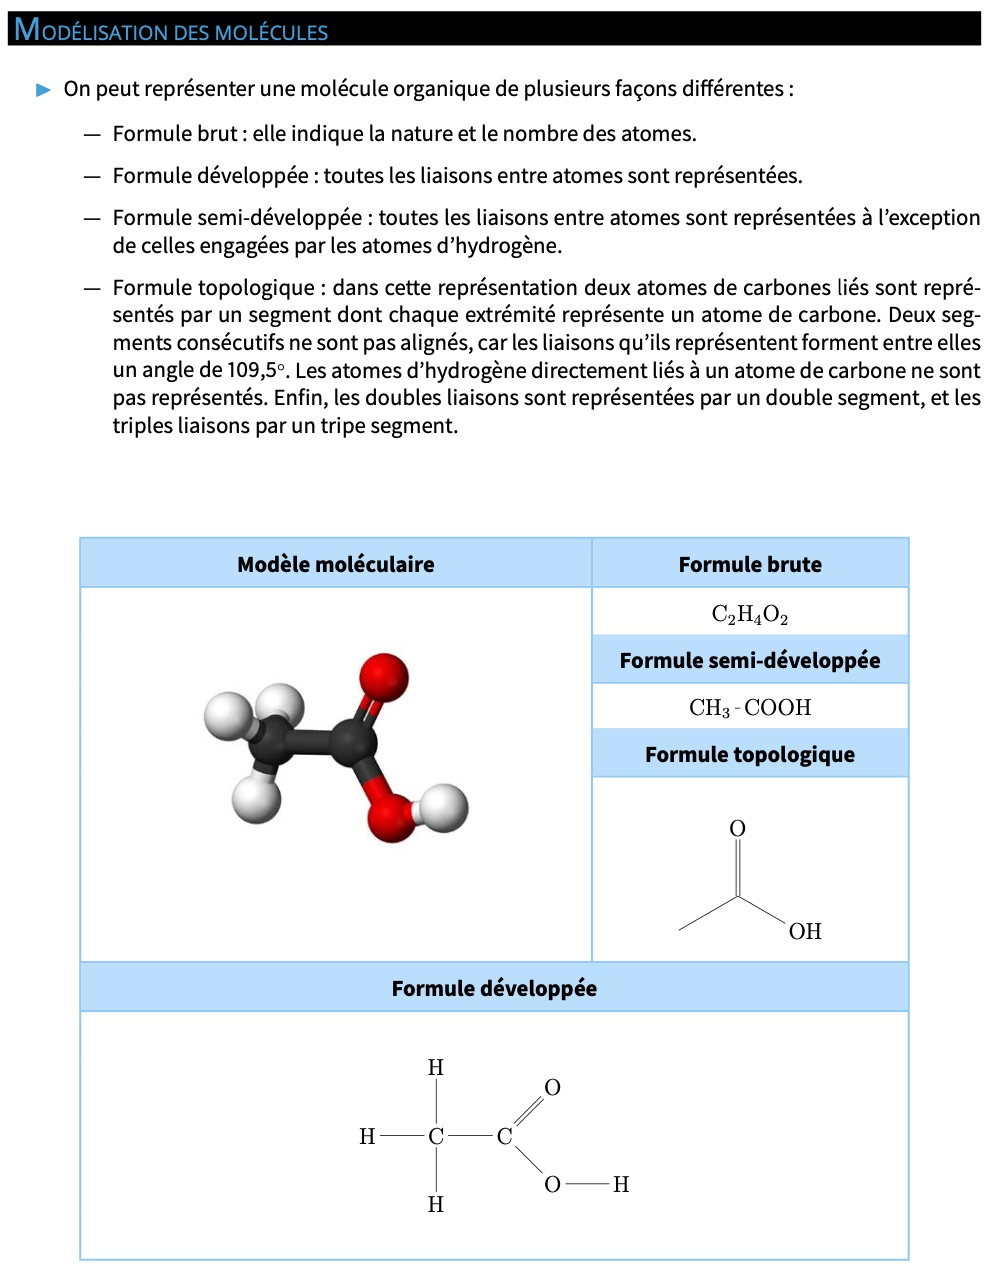
\includegraphics[width=0.6\linewidth]{livre_page2.jpg}
  \caption{\label{} Modélisation de molécules}
\end{figure}

\subsection{Mise en application}

\begin{tcolorbox}[colback=blue!10!white, colframe=blue!75!black, title=Application : Structure électronique]
  Exercices à faire en groupe (dans le livre de Physique) : 
  \begin{itemize}[noitemsep]
    \item N°1
    \item N°2
    \item N°3 page 40
  \end{itemize}
\end{tcolorbox}

\vspace{1em}

\trou{
  \begin{itemize}
    \item 1ere molécule (Acide butanoïque)
    \begin{itemize}[noitemsep]
      \item Formule brute : \ce{C4H8O2}
      \item Formule semi développée : \ce{CH3-CH2-CH2-COOH}
      \item Formule topologique :  \par 
        \chemfig{[:30]--[:-30]-(=[2]O)(-[:-30]OH)}
    \end{itemize}
    \item 2ème molécule (1-propanol)
    \begin{itemize}[noitemsep]
      \item Formule brute : \ce{C3H8O}
      \item Formule semi développée : \ce{CH3-CH2-CH2-OH}
      \item Formule topologique : \par
        \chemfig{[:30]--[:-30]-([:30]OH)}
      \end{itemize}
    \item 3ème molécule 
      \begin{itemize}[noitemsep]
        \item Formule brute : \ce{C8H14O}
        \item Formule semi développée : \ce{CH3-CH2-CH2-CH2-CH2-CO-CH=CH2}
        \item Formule topologique : \par
        \chemfig{[:30]--[:-30]--[:-30]-(=[2]O)-[:-30]=[:30]}
      \end{itemize}
    \item 4ème molécule 
      \begin{itemize}
        \item Formule brute : \ce{C3H602}
        \item Formule semi développée :  \ce{CH3-CH2-COOH}
        \item Formule topologique :  \par 
        \chemfig{[:30]-[:-30]-(=[2]O)-[:-30]OH}
      \end{itemize}

\end{itemize}
}
{\vspace{8em}}

\section{Hydrocarbures / Groupes caractéristiques}

\subsection{Les alcanes}

Les alcanes sont des hydrocarbures aux chaînes carbonées saturées.
\begin{itemize}[noitemsep]
    \item Leur formule brute est \ce{C_{n}H_{2n+2}}.
    \item Le nom d'un alcane est constitué d'un préfixe indiquant le nombre d'atomes de carbone de la chaîne (voir tableau ci-contre), suivi de la terminaison « -ane ».
    \item Exemples :
    \begin{itemize}
        \item Méthane : \ce{CH4}
        \item Éthane : \ce{C2H6}
        \item Propane : \ce{C3H8}
        \item etc.
    \end{itemize}
\end{itemize}

\begin{table}[h]
    \centering
    \begin{tabular}{|c|c|}
    \hline
    Nombre d'atomes de carbone & Racine \\
    \hline
    1 & méthan- \\
    2 & éthan- \\
    3 & propan- \\
    4 & butan- \\
    5 & pentan- \\
    6 & hexan- \\
    \hline
    \end{tabular}
    \caption{Préfixes des alcanes selon le nombre d'atomes de carbone}
\end{table}

\subsection{Les alcènes}

Les alcènes sont des hydrocarbures aux chaînes carbonées insaturées possédant au moins une double liaison carbone-carbone \ce{C=C}.
\begin{itemize}[noitemsep]
    \item Leur formule brute est \ce{C_{n}H_{2n}}.
    \item Le nom d'un alcène est constitué d'un préfixe indiquant le nombre d'atomes de carbone de la chaîne, suivi de la terminaison  "-ène".
    \item Exemples :
    \begin{itemize}
        \item Éthène : \ce{C2H4} ou \ce{CH2=CH2}
        \item Propène : \ce{C3H6} ou \ce{CH3-CH=CH2}
    \end{itemize}
\end{itemize}

\subsection{Composés aromatiques}

\begin{itemize}[noitemsep]
  \item Les composés aromatiques sont des molécules présentant un ou plusieurs cycles, c'est-à-dire que les atomes sont arrangés de façon à former une structure cyclique plane.
  \item Le modèle des hydrocarbures aromatiques est le benzène C6H6, constitué d'un cycle à 6 atomes de carbone formant un hexagone régulier.
\end{itemize}

\begin{figure}[H]
  \centering
  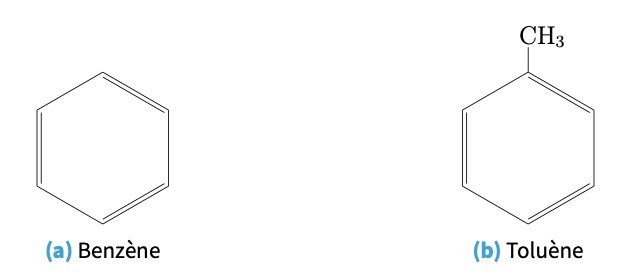
\includegraphics[width=0.7\linewidth]{aromatiques.jpg}
  \caption{\label{} Composés aromatiques}
\end{figure}


\subsection{Groupes caractéristiques}

Dans une molécule organique, on appelle groupe caractéristique, ou groupe fonctionnel, un enchaînement particulier d'atomes dont un au moins n'est ni un carbone, ni un hydrogène.
\begin{itemize}
    \item À un groupe caractéristique donné peut correspondre plusieurs fonctions chimiques. Les composés d'une même fonction chimique ont des propriétés chimiques semblables.
    \item Certaines molécules possèdent plusieurs groupes fonctionnels. On les appelle molécules polyfonctionnelles.
\end{itemize}

\begin{figure}[H]
  \centering
  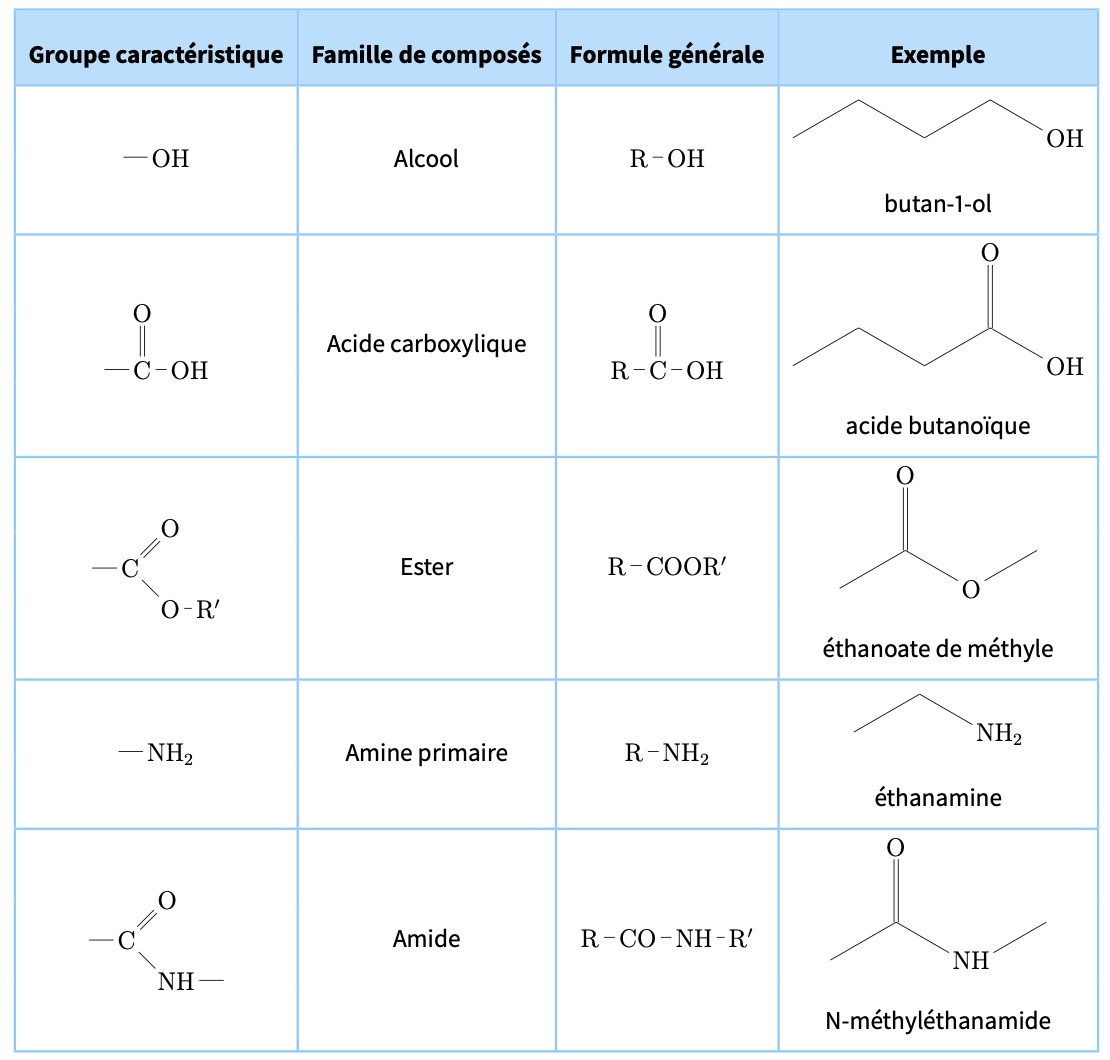
\includegraphics[width=0.7\linewidth]{groupes_fonctionnels.jpg}
  \caption{\label{} Groupes fonctionnels}
\end{figure}

\subsection{Les polymères}

\subsubsection{Définition et propriétés}

On appelle macromolécule, une molécule de masse molaire élevée.
\begin{itemize}[noitemsep]
    \item Un polymère est une macromolécule engendrée par la répétition un grand nombre de fois d'un motif élémentaire appelé \textcolor{blue}{monomère}.
    \item Soit \ce{M} un monomère, le polymère : \ce{M-M-M-M-M} se note ainsi
    \chemfig{\vphantom{M}-[@{op,.75}]M-[@{cl,0.25}]}
    \polymerdelim[delimiters ={[]}, height = 5pt, indice = \!\!n]{op}{cl}
\end{itemize}
\vspace{1em}

\begin{tcolorbox}[colback=blue!10!white, colframe=blue!75!black, title=Propriétés essentielles des polymères et exemples]
  \textbf{Polyéthylène}
\chemfig{\vphantom{CH_2}-[@{op,.75}]CH_2-CH_2-[@{cl,0.25}]}
\polymerdelim[height = 5pt, indice = \!\!n]{op}{cl}
\bigskip

\begin{enumerate}[noitemsep]
  \item Pour un polymère, l'indice de polymérisation est \textbf{le nombre de répétitions du motif élémentaire}.
  \item Plus l'indice de polymérisation est important, plus la viscosité, la température de fusion, la résistance mécanique et la température de transition vitreuse du matériau polymère augmente (jusqu'à une valeur limite).
  \item \textbf{Polymères naturels} : polymères qui existent en l'état, dans la nature
  \begin{itemize}[noitemsep]
    \item Protéines
    \item L'acide nucléique (ADN)
    \item Le caoutchouc
  \end{itemize}
   \item \textbf{Polymères synthétiques} : polymères crées de manière artificielle (dans l'industrie chimique)
   \begin{itemize}[noitemsep]
    \item Le PVC
    \item Polycarbonate
  \end{itemize}
\end{enumerate}

\end{tcolorbox}

\subsubsection{Polyaddition et polycondensation}

\begin{tcolorbox}[colback=blue!10!white, colframe=blue!75!black, title=A connaître par coeur]

\begin{enumerate}[noitemsep]
  \item La transformation permettant de passer d'un monomère à un polymère s'appelle la polymérisation
  \item La polycondensation est une réaction de polymérisation qui se fait avec la génération de petites molécules telles que \ce{H2O}, \ce{HCl} ou \ce{NH3}
  \item La polyaddition est une réaction de polymérisation qui se fait sans \textbf{aucune} génération de petites molécules
\end{enumerate}


\begin{figure}[H]
  \centering
  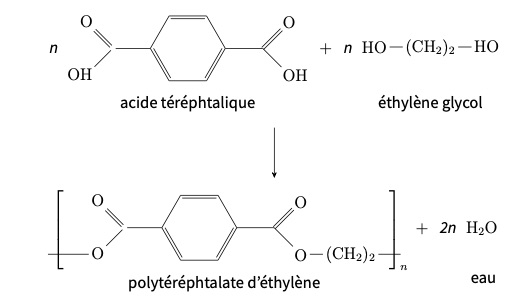
\includegraphics[width=0.7\linewidth]{polycondensation.jpg}
  \caption{\label{} Polycondensation}
\end{figure}

\end{tcolorbox}



\subsection{Application}

\begin{tcolorbox}[colback=blue!10!white, colframe=blue!75!black, title=Application : Structure électronique]
  Exercices à faire en groupe (dans le livre de Physique) : 
  \begin{itemize}[noitemsep]
    \item N°8 (Les peintures) (ne pas donner la formule topologique)
    \item N°12 (Nylon français)
    \item N°13 page 43
    \item Si le temps le permet, faire l'exercice N°2
  \end{itemize}
\end{tcolorbox}



\section{Sources}

Quelques cours / sources intéressantes : 

\begin{itemize}[noitemsep]
  \item \href{https://www.maxicours.com/se/cours/etablir-le-schema-de-lewis-et-la-geometrie-d-une-molecule/}{Maxicours}
  \item \href{https://www.youtube.com/watch?v=bmV-Tbv2Me8&ab_channel=e-profs-PhysiqueChimie}{Vidéo Youtube}
\end{itemize}


\end{document}
